\documentclass[letterpaper,11pt]{article}
\usepackage[margin=1in]{geometry}
\usepackage[T1]{fontenc}
\usepackage[utf8]{inputenc}
\usepackage[english]{babel}
\usepackage{amsmath}
\usepackage{amsfonts}
\usepackage{amssymb}
\usepackage{amsthm}
\usepackage{graphicx}
\usepackage{color}
\usepackage{url}
\usepackage{textcomp}

\title{Homework 2}
\author{Kiera Lavato}
\date{R11808006 | CS-3383}

\newcommand{\notimplies}{%
  \mathrel{{\ooalign{\hidewidth$\not\phantom{=}$\hidewidth\cr$\implies$}}}}

\begin{document}

	\maketitle
	
	\begin{enumerate}
		\item Show that $(A\cup C)\cap(B\cup C) \subseteq (A \cap B) \cup C$
		
		\begin{description}
		    \item $(A\cup C)\cap(B\cup C)$
		    \item $\implies ((A\cup C)\cap B) \cup ((A\cup C)\cap C)$
		    \item $\implies ((A \cap B) \cup (C \cap B) \cup (A \cap C) \cup (C \cap C))$
		    \item $C \cap C \implies C$ 
		    \item $\therefore\implies ((A \cap B) \cup (C \cap B) \cup (A \cap C) \cup C)$
		    \item $\vdots$
		    \item $\{(A \cap B), (C \cap B), (A\cap C), C\}$
		    \item $\implies(A\cap B) \subseteq \{(A \cap B), (C \cap B), (A\cap C), C\}$
		    \item $\implies C \subseteq \{(A \cap B), (C \cap B), (A\cap C), C\}$
		    \item $\therefore (A\cup C)\cap(B\cup C) \subseteq (A \cap B) \cup C$
		\end{description}
		
		\newpage
		\item Let $f:A\mapsto B$. Show that the following relation $R$ is an equivalence relation on $A: (a,b) \in R$ if and only if $f(a)=f(b)$.
		
		A relation $R \subseteq A\times A$ is an equilivence relation if:
		\begin{enumerate}
		    \item It is reflexive.\\
		    $(a,a)\in R$ for every $a \in A$.\\
		    Every node has a self-loop.\\
		    
		    \item It is symmertic.\\
		    $(a,b)\in R$ or $(b,a)\in R$.\\
		    Every edge between two nodes is "two ways".\\
		    
		    \item It is transitive.\\
		    $(a,b)\in R$ and $(b,c)\in R$, then $(a,c)\in R$.\\
		    You can always "shortcut".
		\end{enumerate}
		
		Since $f:A\mapsto B$, we need to prove that $\{A: (a,b) \in R \}$ exists $\iff f(a)=f(b)$. Lets say:
		\begin{description}
		    \item - $f(n)=n^2$
		    \item - $a=1$
		    \item - $b=2$
		\end{description}
		
		The following must be false for $\{A: (a,b) \in R \}$ exists $\iff f(a)=f(b)$:
		\begin{description}
		    \item $f(a)=f(b)$
		    \item $f(a) \implies f: 1\mapsto 1 \therefore f(a) = 1$
		    \item $f(b) \implies f: 2\mapsto 2 \therefore f(b) = 2$
		    \item $f(a)=f(b)\implies a=b \implies 1=2$
		\end{description}
		
		Since $a=b$ where $f(a)=f(b)$, this overall means that each value within one set is mapped directly to another value within the other set. That makes it symmetric, and therefore that makes it an equivalence relation.
		
		
		
		
		
		
		
		
		\newpage
		\item Let $R_1$ and $R_2$ be any two partial orders on the same set $A$. Show that $R_1\cap R_2$ is a partial order.\\\\
		
        A relation $R \subseteq A\times A$ is a partial order if:
		\begin{enumerate}
		    \item It is reflexive.\\
		    $(a,a)\in R$ for every $a \in A$.\\
		    Every node has a self-loop.\\
		    
		    \item It is antisymmertic.\\
		    $(a,b)\in R$ and $a \not= b$, then $(b,a)\not\in R$.\\
		    Every edge between two different nodes is one-way.\\
		    
		    \item It is transitive.\\
		    $(a,b)\in R$ and $(b,c)\in R$, then $(a,c)\in R$.\\
		    You can always "shortcut".
		\end{enumerate}
		
		$R_1, R_2 \subseteq A$. Let's say:
		\begin{description}
		    \item 1. $R_1 = \{(a,b)\}$
		    \item 2. $R_2 = \{(b,c)\}$
		\end{description}
		
		$R_1$ and $R_2$ must be valid for the following:
		\begin{description}
		    \item 1. $a \implies a$, $b \implies b$, and $c\implies c$.
		    \item 2. $a \to b \notimplies b \to a$.
		    \item 3. $(a,b) \cap (b,c) \implies (a,c)$.
		\end{description}
		
		Because all of these things are in-fact possible, $R_1\cap R_2$ is a partial order.
		\newpage
		\item Show that any function from a finite set to itself contains a cycle.\\\\
		Let's say that there are two finite sets:
		\begin{description}
		    \item $s_0=\{ a,b,s_1 \}$
		    \item $s_1=\{ c,d,s_0 \}$
		\end{description}
		Given that $s_1$ is a member of the set $s_0$ and $s_0$ is a member of the set $s_1$, these two sets would be constantly calling themselves, thus being in a loop. Now let's assume that theres two functions instead of two sets.
		\begin{description}
		    \item $f_0(n)=a+b+f_1(n)$
		    \item $f_1(n)=c+d+f_0(n)$
		\end{description}
		
		When $f_0(1)$ is called, for example, there would thus be a constant cycle between the two functions being called. We can try to assume the following:
		
        \begin{description}
		    \item $\forall n \in \mathbb{R}, \exists a,b,c,d \in \mathbb{R}, f_0(n)$ approaches a value such that $f_0(n) \not\in \mathbb{R}$:
		    \item $f_0(n)=a+b+f_1(n)$
		    \item $f_1(n)=c+d+f_0(n)$
		    \item $\implies f_0(n)=a+b+c+d+f_0(n)$
		    \item $\implies f_0(n)-f_0(n)=a+b+c+d$
		    \item $\therefore \forall n \in \mathbb{R}, n \implies 0$
		\end{description}
		Therefore, the constant loop means that the sum approaches an unreal value. This means that the two sets will continuously loop on themselves, constantly adding itself to its own function.
		This means that any function from a finite set contains a cycle (which could potentially repeat infinite times.)
		
		
		
		\newpage
		\item Construct a Deterministic Finite Automata accepting each of the following:
		\begin{description}
			\item a) $\{w\in \{a,b\}^*:w \text{ has } abab \text{ as a substring}\}$\\\\
			Where the initial state is $f_0$ and the final state is $f_4$.\\
			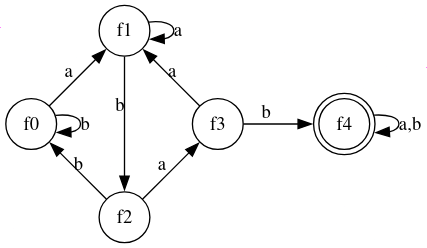
\includegraphics[scale=0.7]{/home/kiki/Downloads/5.1.png}
			
			\item b) $\{w\in \{a,b\}^*:w \text{ has neither } aa \text{ nor } bb \text{ as a substring}\}$\\\\
			Where the initial state is $f_0$ and the final state is $f_1$ or $f_2$.\\
			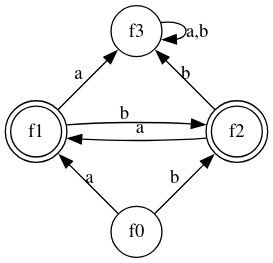
\includegraphics[scale=0.7]{/home/kiki/Downloads/5.2.png}
			
			
			
		\end{description}
	\end{enumerate}
\end{document}